% Chapter 1

\chapter{Introduction} % Main chapter title

\label{Chapter1} % For referencing the chapter elsewhere, use \ref{Chapter1} 

%----------------------------------------------------------------------------------------

\section{Background to the problem}
A software system is constantly subject to change pressure from its environment, therefore it needs to evolve to deliver value to its stakeholders throughout its lifetime: it has been regarded at least since the 1980's that software evolution is the most expensive part of the software lifecycle \citep{Lehman1980a}. Therefore, an understanding of the capacity of a system to adapt to changes in its environment can impact on the software production process \citep{Yu2006a}.

Open source development challenges traditional best practices in software development by blurring the difference between users and developers \citep{Hippel2003}. The open source development model originated in the academic community and has transcended into private enterprise, where in many cases it has proven an efficient alternative to strong intellectual property protection \citep{Kogut2001a}.

Common tasks in software evolution include cloning, branching and merging of the code base; in addition to these processes, the open source license grants the freedom to fork a project: open source projects can evolve in parallel, splitting in two or more different projects, steered by different development teams.

The gain in popularity of the open source development model has brought forward the importance of understanding forking processes. \citet{Kogut2001a} argue that forking results in competing versions of the original project and that forking is therefore a major failure risk for open source projects. \citet{Nyman2013a} argue that forking is a remedy against ailments of proprietary software (planned obsolescence, vendor lock-in, hostile takeovers, etc.) and that forking facilitates experimentation. \citet{Robles2012a} suggest that a purposeful fork can solve technical-, license- and team-related problems by restoring the balance between the stakeholders of a project. Therefore, a controversy exists within the software engineering community, whether forking is a risk or an opportunity.

%----------------------------------------------------------------------------------------

\section{Justification for the research}

Concepts in software evolution and biological evolution are often described using a common vocabulary \citep{Yu2006a}, so it seems natural to look at evolutionary biology for potential methods to solve this controversy.

\citet{Lehman1980a} postulates that there are recurring patterns which govern software evolution, independently of the decisions taken by individual managers and programmers. Therefore, software evolution might, as biological evolution, be understood as a process which is not designed, but resulting from characteristics inherent to a population: A population need not be composed of biological entities, characteristics need not be encoded in DNA and the environment can be artificial, thus the term "evolution" can be used to describe processes in different domains, as long as the population considered ensures its own perpetuation \citep{Nehaniv2006a}. If the term “software system” is taken to encompass a system's infrastructure, code base and community of developers \citep{Yu2006a}, then a software system is capable of sustaining itself, and thus the change processes affecting a population of software releases can be described as evolution (figure \ref{fig:evolution}).

\begin{figure}[H]
  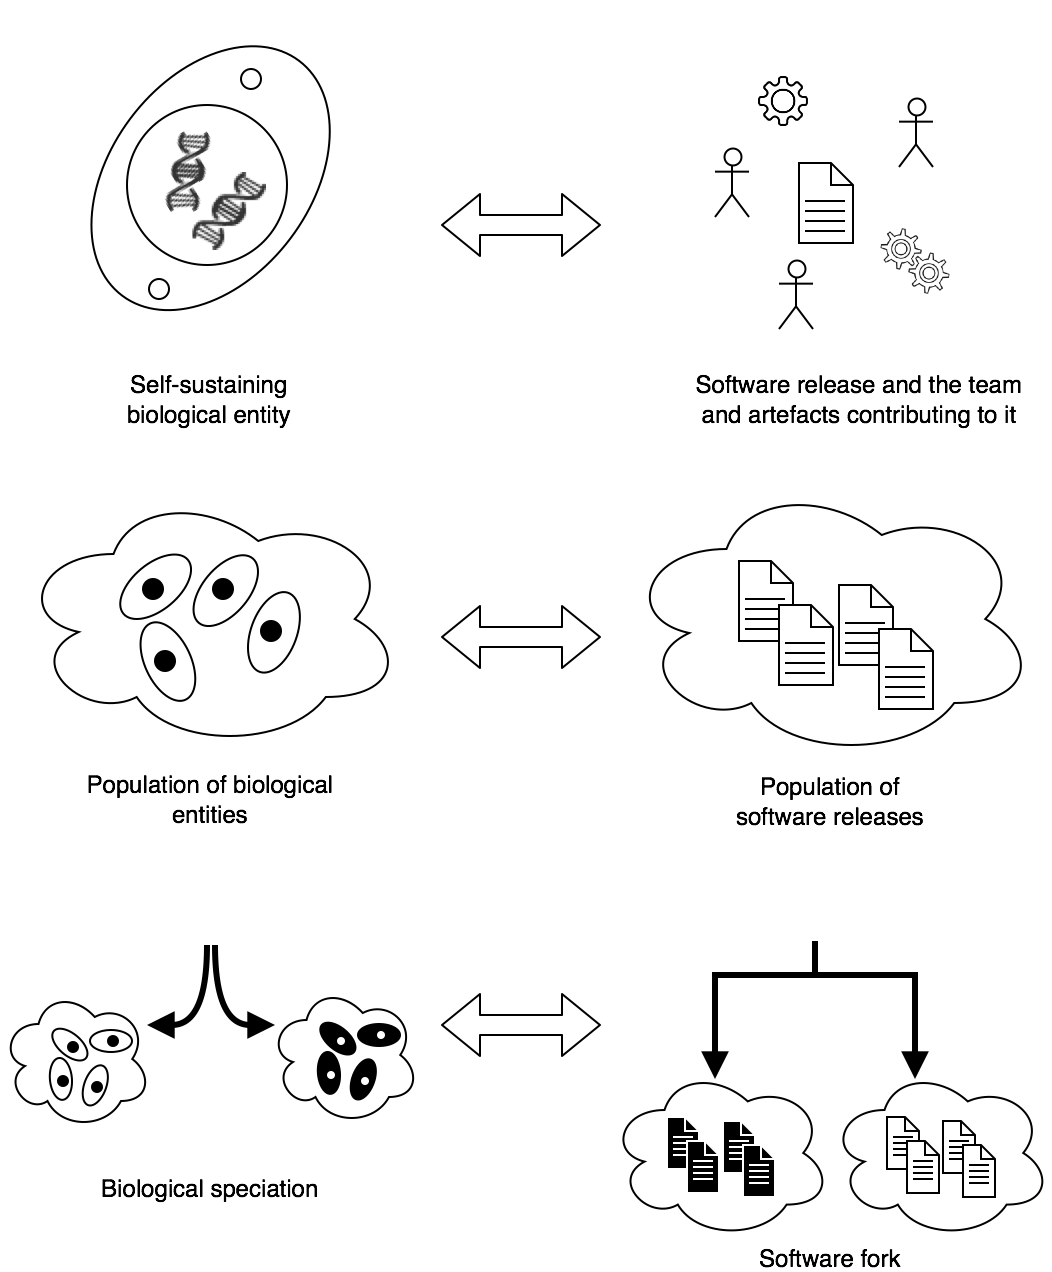
\includegraphics[width=\textwidth]{evolution.png}
  \caption{A comparative diagram between biological and software evolution.}
  \label{fig:evolution}
\end{figure}

%----------------------------------------------------------------------------------------

\section{Definitions}

Based on the work by \citet{Robles2012a} a working definition of a fork can be formulated as follows:

\definition{Fork}{A fork is a bifurcation from an existing project, resulting in an autonomous development strand, with its own name, infrastructure, code base and community of developers.}

\noindent
Based on the work by \citet{Nehaniv2006a} and \citet{Yu2006a}, a working definition of the evolution of software can be formulated as follows:

\definition{Software evolution}{The evolution of software is a process which affects a population of software releases. Software releases are characterized by code and organizational resources. Software evolution is distinct from the governance of a software project, as software evolution is independent of the decisions taken by individual managers and programmers.}

%----------------------------------------------------------------------------------------

\section{Scope of the research}

Forking is a process explicitly enabled by open source software licenses; forking is contrary to strong intellectual property protection; therefore the scope of the research is limited to open source software. Software forks are known to have occurred in the areas of networking, web applications, development environments, multimedia, games, operating- and desktop- systems, utilities, graphics software, databases, enterprise resource planning, security and package management \citep{Robles2012a}, thus affecting a large portion of the software development domain.

Some projects that have gained a large user base originated from forks, for example the MariaDB database engine, the Android operating system and the LibreOffice suite of office applications, forked for different reasons and with different outcomes. Rather than trying to gain a comprehensive overview of the impact of forking on software development, a task that was undertaken by \citet{Robles2012a}, the present research examined three forks: MySQL / MariaDB, Linux / Android and OpenOffice / LibreOffice. Data was collected from the projects' online repositories, without interacting directly with the developers (“third degree data”). This approach entails that data cannot be controlled nor its quality be assessed through other means, therefore, the availability and completeness of the data archived in the repositories was a factor that played an important role in the choice of projects to examine.

Using real-world case studies for describing a software development situation has been practiced in computer science, and it is possible to empirically test hypotheses using this approach \citep{Runeson2009b}. Hypotheses were formulated as research questions, presented in paragraph 2.1.

%----------------------------------------------------------------------------------------

\section{Aim}
Any organization aiming to adopt open source software development might face a fork situation during the software's lifecycle, or might decide to fork existing software as a means to solve technical-, license- and team-related problems or to facilitate experimentation, as suggested by \citet{Robles2012a}. The aim of this research is to gain empirical evidence of whether phylogenetic methods from evolutionary biology can quantify the risks and opportunities associated with software forking processes.

To this end, the present research reviewed the current state of literature on forking, selected suitable open source software repositories to collect data and implemented selected phylogenetic methods using appropriate libraries. An attempt was made to advance the understanding of forking processes by answering the research questions detailed in chapter 2.

%----------------------------------------------------------------------------------------

\section{Outline of the dissertation}
The rest of the dissertation is organized as follows: chapter 2 defines the research questions, reviews existing literature and examines the objectives in detail. Chapter 3 examines the data acquisition process, justifies the choice of phylogenetic techniques and relates the chosen statistical techniques to the research questions. Chapter 4 details how the data was acquired, processed using phylogenetic techniques and analysed using statistical techniques. Chapter 5 concludes, delineates possible further research and reflects on the research process as it was carried out.
